\chapter[Целочисленная арифметика. Массивы]{Семинар 04. Целочисленная арифметика. Одномерные и многомерные массивы. Простые алгоритмы}

Целью семинара изучение команд, обеспечивающих обработку целочисленных данных со знаком и без знака, организацию управления в программах, использующих целочисленную арифметику. Распределение памяти под целочисленные одномерные и многомерные массивы, организации доступа к элементам массивов различной размерности.

Проведение семинара предполагается по следующему плану:
\begin{enumerate}
    \item Обзор команд, обеспечивающих поддержку целочисленной арифметики.
    \item Организация в памяти одномерных массивов и методы доступа к этим массивам.
    \item Примеры работы с одномерными массивами.
\end{enumerate}

\section{Сценарий семинара}


\subsection{Обзор команд, обеспечивающих поддержку целочисленной арифметики}

Предлагается кратко охарактеризовать список основных и дополнительных команд процессора, реализующих базовую арифметику и логику для 32-х разрядной архитектуры. В конспекте лекций я их разбил на отдельные небольшие таблицы. Думаю, что после завершения перевода они перенесутся в методу для самостоятельной работы (сами списки взяты из системы помощи RARS).

Но в целом понятно, что на все эти команды разом обращать внимание бесполезно поэтому проще продемонстрировать те схемы, которые в сокращенном виде представляют команды процессора. Одна из них --- это список команд в эмуляторе RARS (рисунок~\ref{ref-rars-commands}). При необходимости их описание можно прочитать в системе помощи эмулятора.

\begin{figure}[htbp]
    \centering
    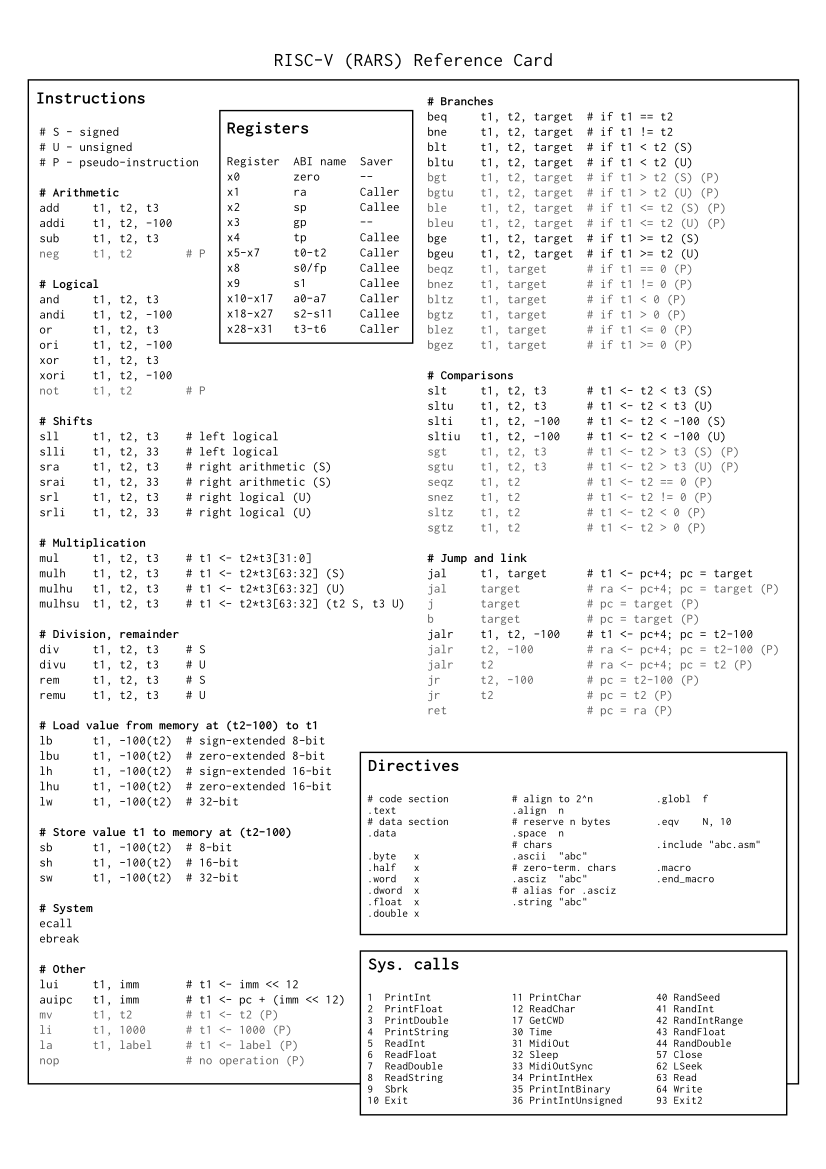
\includegraphics[width=1.0\textwidth]{img/RARS_reference_card.png}
    \caption{Команды 32-разрядного процессора RISC-V, реализованные в эмуляторе RARS}
    \label{ref-rars-commands}
\end{figure}

Другая схема дает более полное описание уже не только RV32I, но и других вариантов. Но там легко выделить изучаемый процессор. И возможно, что она является более наглядной. Занимает, правда две страницы (рисунок~\ref{ref-riscv-commands-01} и рисунок~\ref{ref-riscv-commands-02}). Основное достоинство --- более четко расписаны операнды и приводятся типы форматов команд. Но в целом на больше будет интересовать первый документ.

\begin{figure}[htbp]
    \centering
    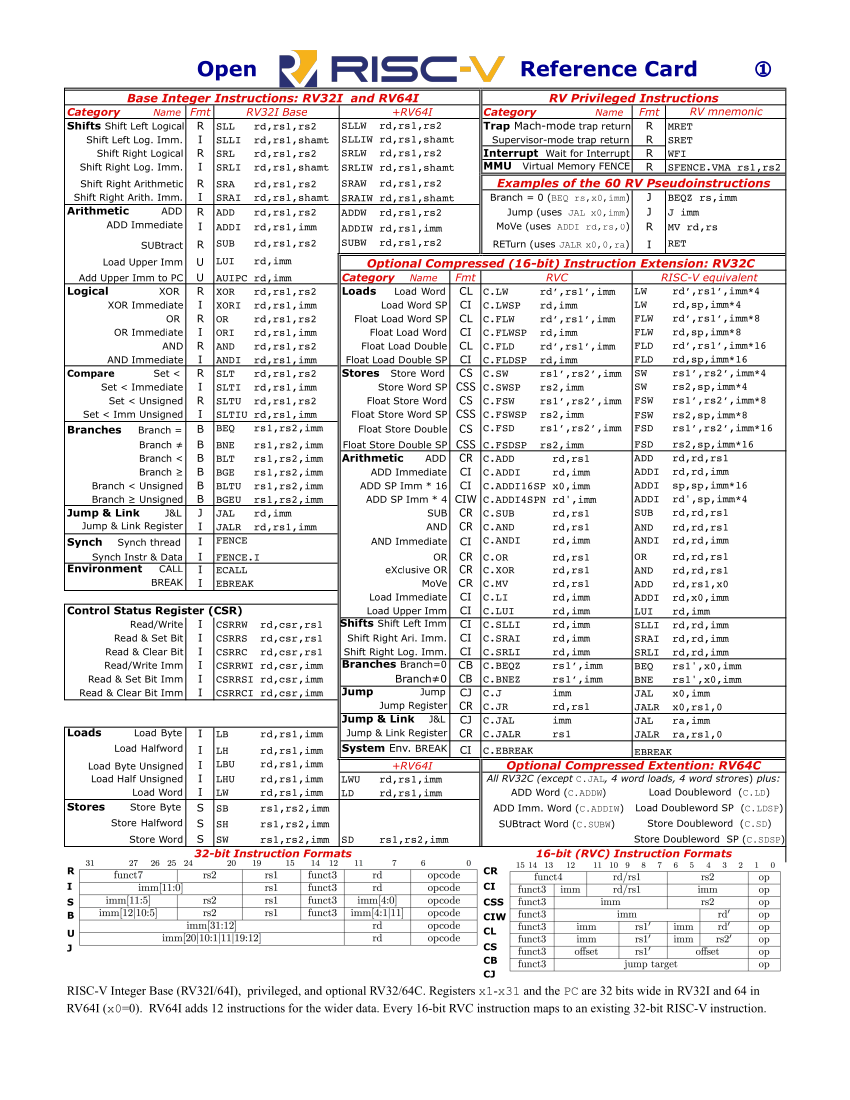
\includegraphics[width=1.0\textwidth]{img/riscv-reference-card-01.png}
    \caption{Команды процессора RISC-V (начало)}
    \label{ref-riscv-commands-01}
\end{figure}

\begin{figure}[htbp]
    \centering
    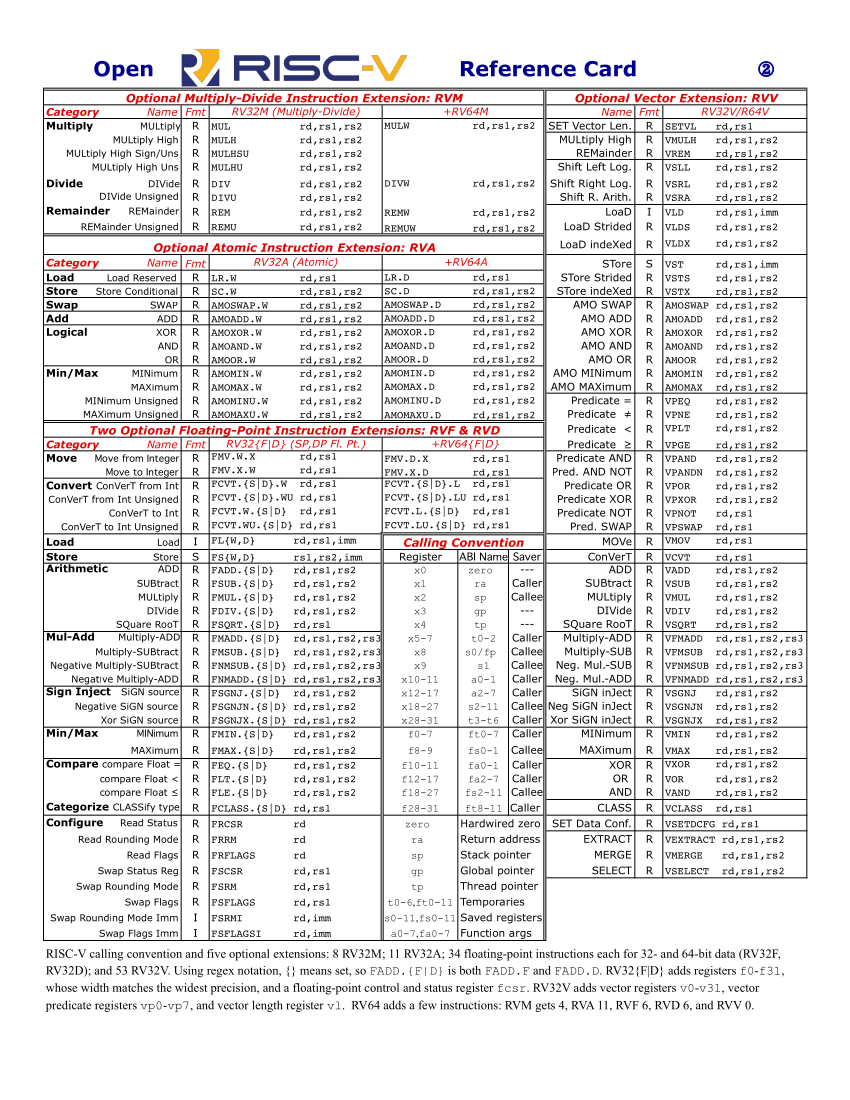
\includegraphics[width=1.0\textwidth]{img/riscv-reference-card-02.png}
    \caption{Команды процессора RISC-V (окончание)}
    \label{ref-riscv-commands-02}
\end{figure}

Обе схемы выложены в LMS. Поэтому при необходимости их можно будет скачать. В принципе на второй схем можно пояснить, что команды целочисленного умножения и деления являются для 32-х разрядной архитектуры опциональными (не знаю, насколько это важно).

Основная идея --- сказать, чтобы не пугались, что их много. Не все будут нужны и не сразу, а постепенно. Главное - ориентироваться в базовом списке в основных группах и при необходимости читать о них в системе помощи.

Лалее по ходу объяснения можно обращаться к различным группам команд, когда потребуются различия в представлении:
\begin{itemize}
    \item знаковых и беззнаковых чисел;
    \item байтов, слов, двойных слов;
    \item и т.д.
\end{itemize}

\section{Организация в памяти одномерных массивов и методы доступа к этим массивам}

Изначально можно представить простую программу на Си, в которой, как и в последующей ассемблерной решается задача формирования и вывода элементов целочисленного массива:

\begin{verbatim}
    #include <stdio.h>

    int array[16];

    int main()
    {
        fill:
        for(int i = 0; i < 16; ++i) {
            array[i] = i+1;
        }
        printf("--------\n");
        out:
        for(int i = 0; i < 16; ++i) {
            printf("%d\n", array[i]);
        }
        return 0;
    }
\end{verbatim}

\subsection{Работа с одномерными массивами}
Можно начать с пояснения того, что формирование индекса элемента массива как отдельно рассматриваемого целого числа, увеличивающегося на 1 в принципе возможно. Однако в ассемблере предпочтительнее манипулировать непосредственно с адресным пространством нужной величины, а не умножать каждый раз на величину слова, так как операция умножения затратна по времени. Она даже не входит в базовый набор. Хотя можно ислпользовать сдвиги вместо умножения. Но все равно это лишние команды (но при желании пусть используют).
Основной режим работы - использование косвенной адресации с индексацией относительно начала массива.

Показать, что для выделения массива достаточно задать память, выделяемую под него различными способами:
\begin{itemize}
    \item можно выделить пространство требуемого размера;
    \item при наличии заранее предопределенных значений элементов можно их перечислить;
    \item при неизвестном числе элементов можно зарезервировать некоторый большой кусок памяти, а количество элементов задавать числом, меньшим выделенного размера, которое (как и впрограмме на Си) может служить окраничителем цикла при формировании массива;
    \item можно выделить память под массив на куче после получения числа элементов в массиве.
\end{itemize}
В качестве стартового примера можно опять обратиться к лекциям Г. Курячего:
\begin{verbatim}
.data
sep:    .asciz  "--------\n"    # Строка-разделитель (с \n и нулём в конце)
.align  2                       # Выравнивание на границу слова
array:  .space  64              # 64 байта
arrend:                         # Граница массива
.text
la      t0 array                # Счётчик
la      s1 arrend
li      t2 1            # Число, которое мы будем записывать в массив
fill:   sw      t2 (t0)         # Запись числа по адресу в t0
addi    t2 t2 1         # Изменим число
addi    t0 t0 4         # Увеличим адрес на размер слова в байтах
bltu    t0 s1 fill      # Если не вышли за границу массива
la      a0 sep          # Выведем строку-разделитель
li      a7 4
ecall
la      t0 array
out:    li      a7 1
lw      a0 (t0)         # Выведем очередной элемент массива
ecall
li      a7 11           # Выведем перевод строки
li      a0 10
ecall
addi    t0 t0 4
blt     t0 s1 out
li      a7 10           # Останов
ecall
\end{verbatim}
На основе этого примера можно пояснить, что при выделении под массив, который заполняется полностью, можно не использовать его размерность, а указывать метку, задающую ограничительный адрес.

На примере этой программы можно предложить модификации на занятиях, в которых заполнение осуществляется побайтно и по 16 разрядным словам (эти примеры лежать не будут, студенты должны сделать самостоятельно). При этом следует откорректировать не только команду загрузки в память, но и чтения из нее (при выводе).

Пример для генерации байтового массива:
\begin{verbatim}
    .data
    sep:    .asciz  "--------\n"    # Строка-разделитель (с \n и нулём в конце)
    .align  2                       # Выравнивание на границу слова
    array:  .space  64              # 64 байта
    arrend:                         # Граница массива
    .text
    la      t0 array                # Счётчик
    la      s1 arrend
    li      t2 1            # Число, которое мы будем записывать в массив
    fill:   sb      t2 (t0)         # Запись числа по адресу в t0
    addi    t2 t2 1         # Изменим число
    addi    t0 t0 1         # Увеличим адрес на размер слова в байтах
    bltu    t0 s1 fill      # Если не вышли за границу массива
    la      a0 sep          # Выведем строку-разделитель
    li      a7 4
    ecall
    la      t0 array
    out:    li      a7 1
    lb      a0 (t0)         # Выведем очередной элемент массива
    ecall
    li      a7 11           # Выведем перевод строки
    li      a0 10
    ecall
    addi    t0 t0 1
    blt     t0 s1 out
    li      a7 10           # Останов
    ecall
\end{verbatim}
Аналогично можно быстро сделать модификацию и для 16-разрядных слов, изменяя только команды чтения и записи в память.

Помимо этого можно предложиеть модифицировать первую программу так, чтобы вводить в память ограниченное число элементов, заданных максимально допустимым числом. По примеру следующей программы на Си:
\begin{verbatim}
#include <stdio.h>

int array[16];
int n;

int main()
{
    in:
    printf("n = ? ");
    scanf("%d", &n);
    if(n > 16 || n < 1) {
        printf("n = %d is incorrect!\n", n);
        return 1;
    }
    fill:
    for(int i = 0; i < n; ++i) {
        array[i] = i;
    }
    printf("--------\n");
    out:
    for(int i = 0; i < n; ++i) {
        printf("%d\n", array[i]);
    }
    return 0;
}
\end{verbatim}
В этом случае может получиться примерно такое (но необязательно одинаково, так как возможны варианты):

\begin{verbatim}
    .data
    sep:    .asciz  "--------\n"    # Строка-разделитель (с \n и нулём в конце)
    prompt: .asciz  "n = ? "         # Подсказка для ввода числа
    error:  .asciz  "incorrect n!\n"  # Сообщение о некорректном вводе
    .align  2                       # Выравнивание на границу слова
    n:	.word	0		# Число введенных элементов массива
    array:  .space  64              # 64 байта
    .text
    in:
    la 	a0, prompt      # Подсказка для ввода числа элементов массива
    li 	a7, 4           # Системный вызов №4
    ecall
    li      a7 5            # Системный вызов №5 — ввести десятичное число
    ecall
    mv      t3 a0           # Сохраняем результат в t3 (это n)
    ble     t3 zero fail    # На ошибку, если меньше 0
    li      t4 16           # Размер массива
    bgt     t3 t4 fail      # На ошибку, если больше 16
    la	t4 n		# Адрес n в t4
    sw	t3 (t4)		# Загрузка n в память на хранение

    la      t0 array        # Указатель элемента массива
    li      t2 1            # Число, которое мы будем записывать в массив
    fill:   sw      t2 (t0)         # Запись числа по адресу в t0
    addi    t2 t2 1         # Изменим число
    addi    t0 t0 4         # Увеличим адрес на размер слова в байтах
    addi    t3 t3 -1        # Уменьшим количество оставшихся элементов на 1
    bnez    t3 fill         # Если осталось больш 0
    # bltu    t0 s1 fill      # Если не вышли за границу массива
    la      a0 sep          # Выведем строку-разделитель
    li      a7 4
    ecall

    lw	t3 n		# Число элементов массива
    la      t0 array
    out:    li      a7 1
    lw      a0 (t0)         # Выведем очередной элемент массива
    ecall
    li      a0 '\n'         # Выведем перевод строки
    li      a7 11
    ecall
    addi    t0 t0 4
    addi    t3 t3 -1        # Уменьшим количество оставшихся элементов на 1
    bnez    t3 out          # Если осталось больше 0
    # blt     t0 s1 out
    li      a7 10           # Останов
    ecall
    fail:
    la 	a0, error       # Сообщение об ошибке ввода числа элементов массива
    li 	a7, 4           # Системный вызов №4
    ecall
    li      a7 10           # Останов
    ecall
\end{verbatim}

\debate[Примечание.]{На самом деле у меня на отработку этой простой программы ушло немало времени, включая отладку. Возможно стоит, после небольшой паузы, просто продемонстрировать ее решение. Нужно прикинуть хронометраж. Также решил убрать работу с многомерными массивами. Их не будет в задании. Вряд ли на стоит заострять внимание.}

\section{Домашнее задание}

\subsection{До 8 баллов}

Написать программу, осуществляющую суммирование целочисленных элементов одномерного массива. Количество элементов в массиве может варьироваться от 1 до 10. Сами элементы вводятся с клавиатуры. Значение суммы также выводится в консоль эмулятора RARS. Необходимо контролировать, чтобы число вводимых элементов не превышало максимально допустимое. В случае, когда возникает переполнение, необходимо вывести последнее корректное значение суммы и число просуммированных при этом элементов. Суммирование осуществлять после размещения массива в памяти.

\subsection{Опционально до +2 баллов}

Подсчитать количество четных и нечетных элементов в обрабатываемом массиве. Подсчет осуществлять в массиве, который уже расположен в памяти.